\section{方法}

\begin{figure*}[t]
  \centering
  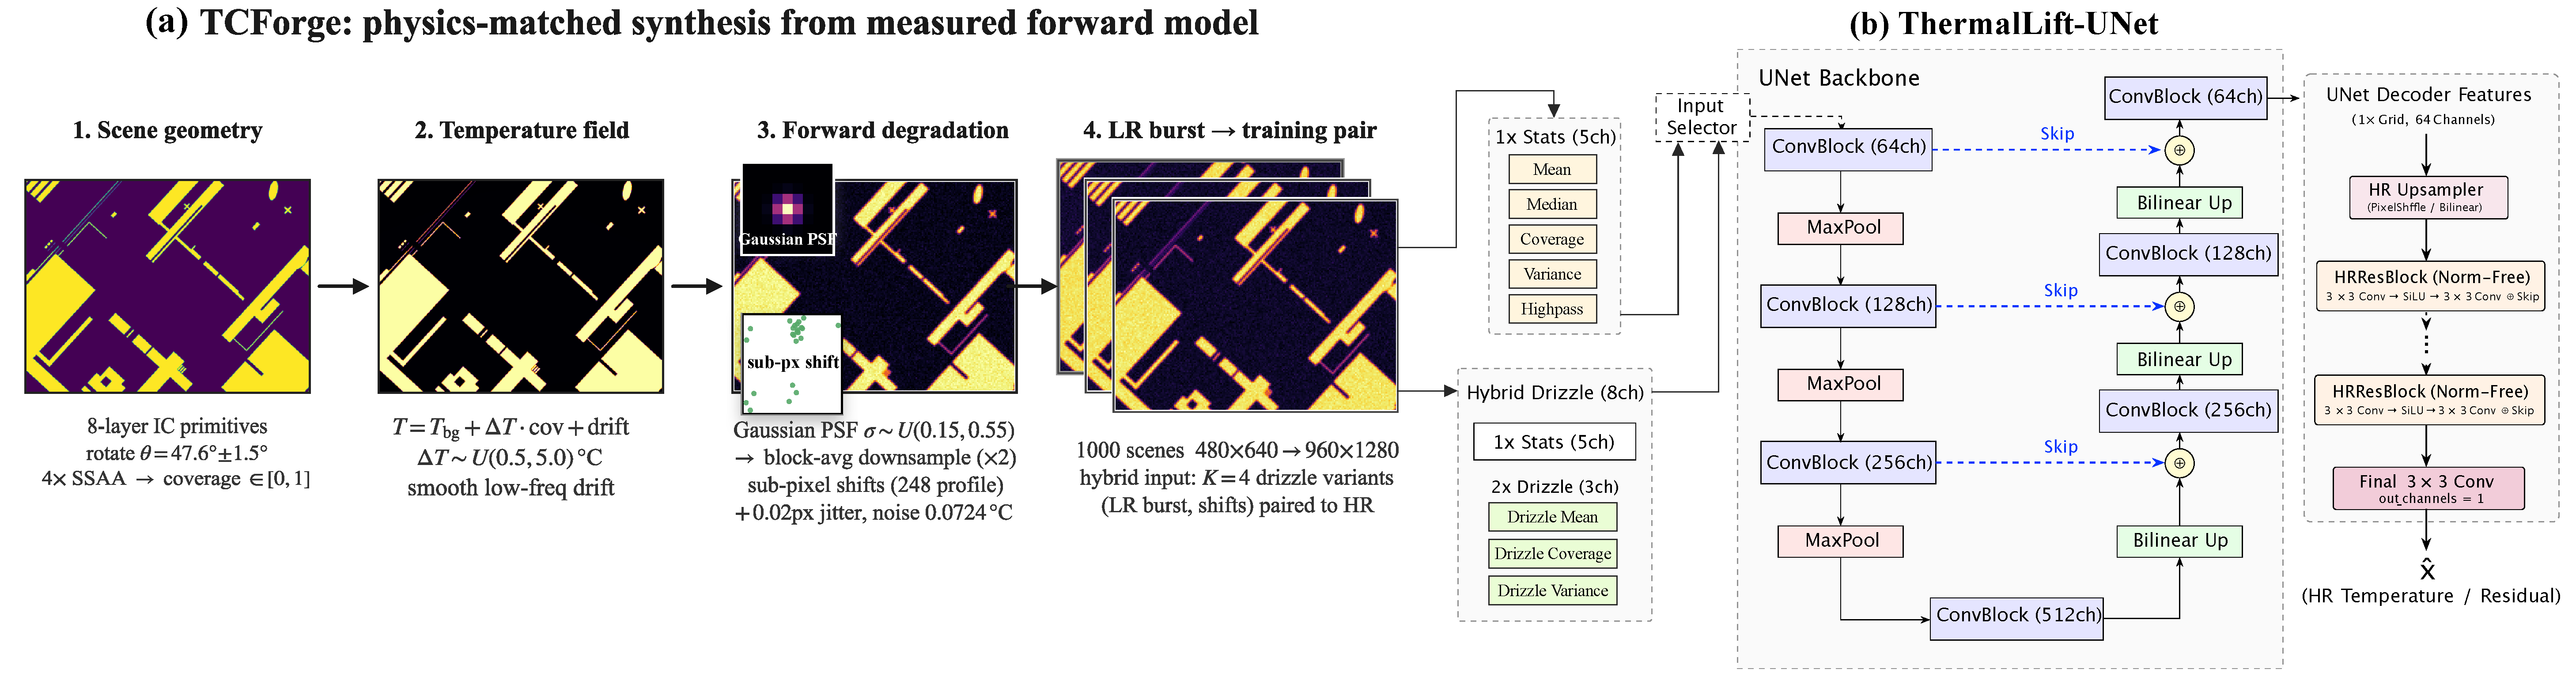
\includegraphics[width=\textwidth]{../figures/fig_tcforge_pipeline.pdf}
  \caption{(a) \eng{TCForge} 物理匹配合成管线：以标定前向模型为核心，
    经 场景几何$\to$温度场渲染$\to$前向退化$\to$训练对 四阶段生成合成训练数据；
    (b) \eng{ThermalLift-UNet} 网络结构：左侧为输入选择器（\(1\times\) 统计 5 通道
    或 \eng{hybrid drizzle} 8 通道），中部为共享 \eng{UNet} 骨干，
    右侧为无归一化高分残差细化模块与最终 \eng{HR} 温度/残差输出。}
  \label{fig:method-pipeline}
\end{figure*}

\subsection{方法概览}

本文方法由三部分组成。首先，以经典重建方法作为验收基准：学习类方法须同时在
\eng{FRC} 频带一致性与锯齿走线剖面指标上不劣于经典基准，方可采纳。
其次，构建参数全部来自实测标定的物理匹配合成平台 \eng{TCForge}，用于合成域训练与真实域部署。
最后，在固定骨干网络下系统变换输入信息通路与观测锚定方式，
组合为
\(\{\text{1x stats},\text{hybrid drizzle}\}\times\{\text{none},\text{band},\text{full},\text{native}\}\)
共 8 种消融配置，以隔离相位证据送达路径与损失侧锚定各自的作用。
图~\ref{fig:method-pipeline} 概括 \eng{TCForge} 合成管线与 \eng{ThermalLift-UNet} 网络结构。
训练端点往往对应最差可交付检查点，因此检查点选取本身是方法的组成部分而非事后修饰；
具体协议详见补充材料。

\subsection{经典重建基准}

\paragraph{Drizzle.}
将 248 帧按轮廓精修位移对齐后，以通量守恒的亚像素散射 \cite{fruchter2002drizzle}
投射到 \(2\times\) 网格（像素分数\(=0.7\)，方形核），覆盖率 \(<1.0\) 的像素置 \eng{NaN}。
\eng{Drizzle} 作为最小假设融合基线，同时暴露细网格方案必须管理的覆盖率与格点伪影风险。

\paragraph{MAP-TV 基准.}
在全部 248 帧上构建 \(S\!\to\!H\!\to\!B\!\to\!D\) 前向模型，采用 \eng{GPU FISTA} \cite{beck2009fast}
配合平滑 \eng{TV} 梯度优化。正则与 PSF 参数由分半代理指标选择（详见补充材料 C）。
该基准作为验收基准，学习类方法须在关键指标上不劣于此方可采纳。

\paragraph{各向异性 coverage-weighted TGV.}
Raster 采集导致行内/行间约束不对称，标准 \eng{TGV} 产生条纹。我们做两项适配：对偶投影改为各向异性椭圆以减弱 \(Y\) 向过强正则，数据梯度按预计算覆盖率加权。两项改动将 artifact score 从 3.870 降至 0.695（\(-82\%\)），raw-control correlation 从 0.902 提升至 0.916。

%% ================================================================
%%  TCForge — 重写：去除花哨小标题，展开核心设计选择
%% ================================================================
\subsection{物理匹配合成平台 TCForge}
\label{sec:tcforge}

学习类热成像超分辨方法面临的核心数据困难是：真实场景不存在像素对齐的高低分辨率训练对。
常见做法有两类——从自然图像出发施加简化退化（如双三次下采样），
或让网络同时估计退化核与重建结果（盲超分）。前者的退化模型与真实物理过程差距显著，
后者在微扫描成像这类高度结构化的退化下缺乏足够约束。
\eng{TCForge} 采取第三条路径：直接复用第~3 节标定的前向物理模型
\(y = D \cdot B \cdot H \cdot S \cdot x + n\) 作为退化生成器。
由此，合成域与真实域共享同一套 PSF、探测器积分、亚像素位移参数，
域差距仅来自场景内容分布，而非退化模型本身。
这一特性使得在合成数据上训练的网络可直接部署于真实采集，
无需额外的域自适应或退化估计步骤。

合成管线分为四个阶段（图~\ref{fig:method-pipeline}(a)）。

\paragraph{场景几何与温度场.}
场景由 8 层随机几何原语（矩形块、条形走线、L 形拐角、焊盘、过孔等）
逐层叠加构造，模拟集成电路版图的典型空间结构。
整体旋转角围绕标定值 \(\theta = 47.6^\circ\) 以 \(U(-1.5^\circ, +1.5^\circ)\) 抖动，
匹配实测光栅扫描几何。为消除旋转后 HR 目标中的阶梯锯齿，
默认启用 \(4\times\) 超采样抗锯齿（SSAA）：在 \(4\times\) 画布渲染后
以 \(4\times4\) 均值下采样，使覆盖率取值连续于 \([0,1]\)。
几何掩模随后渲染为物理温度场：
\begin{equation}
  T = T_{\mathrm{bg}} + \Delta T \cdot \mathrm{coverage}
      + A_{\mathrm{drift}} \cdot \mathrm{smooth\_noise},
\end{equation}
其中温差 \(\Delta T \sim U(0.5, 5.0)\,^\circ\)C 覆盖实测对比度范围，
低频漂移项模拟热背景非均匀性。
噪声按实测均值 \(0.0724\,^\circ\)C 的 lognormal 分布采样，
以匹配真实传感器的噪声统计特征。

\paragraph{前向退化与位移重放.}
对 HR 温度场依次施加：(1) 标定高斯 PSF 模糊，
\(\sigma_{\mathrm{PSF}}\) 在标定可信区间 \([0.15, 0.55]\) LR 像素内均匀采样；
(2) 块均值下采样至 \(1\times\) 网格（模拟 \(10\,\mu\mathrm{m}\) 探测器积分）；
(3) 按实测 248 帧轮廓精修位移 profile 进行亚像素平移重放，
并叠加 \(\sigma_j = 0.02\) px 抖动以增强鲁棒性；
(4) 加入与标定一致的读出噪声。
该退化链的每一步参数均直接取自标定结果而非人工假设，
从而保证合成 burst 与真实采集在 PSF 宽度、探测器响应、
帧间位移分布及噪声水平上保持一致。

\paragraph{训练池构建.}
当前训练池包含 1000 个场景（\(480\times640 \to 960\times1280\)），
每个场景生成完整 LR burst 帧序列及对应 HR 真值。
此外，每个场景预生成 \(K=4\) 种 drizzle 变体供 hybrid 输入使用：
\(k\!=\!0\) 为使用全部帧且无噪声的标准版本，
\(k\!=\!1\text{--}3\) 随机保留 60\%--100\% 帧并注入
\(N(0, 0.05\,\text{px})\) 位移扰动，
以模拟不同质量的观测条件（具体实现见补充材料 C.1）。

%% ================================================================
%%  学习类方法族 — 重写：减少加粗，结构更连贯
%% ================================================================
\subsection{学习类方法族 ThermalLift-UNet}
\label{sec:learning-family}

本节介绍基于学习的重建方法族 \eng{ThermalLift-UNet}。
所有变体共享同一 \eng{UNet} 骨干网络，仅在两个维度上存在差异：
输入信息通路（\(1\times\) 统计输入 vs.\ hybrid drizzle 输入）
与观测锚定方式（无锚定、高频/全频前向一致性、残差参数化）。
据此，各变体分别记为
Stats、Stats+HP-FC、Stats+Full-FC、Hybrid、Hybrid+Native-FC 与 Hybrid+ResObs。

\paragraph{网络结构.}
如图~\ref{fig:method-pipeline}(b) 所示，骨干为标准 \eng{UNet} \cite{ronneberger2015unet}，
基础通道数 \(c=64\)，编码端经 3 次 MaxPool 逐级扩展为 \(c, 2c, 4c, 8c\)，
每个 ConvBlock 包含 \(2\times 3\!\times\!3\) 卷积、GroupNorm \cite{wu2018group}、
SiLU 激活与 SE 通道注意力 \cite{hu2018squeeze}。
解码端通过双线性上采样与跳跃连接恢复空间分辨率。
在解码器特征上采样至 HR 空间后，网络追加两层无归一化的高分残差细化块
（HRResBlock，图~\ref{fig:method-pipeline}(b) 右侧），
每块包含 \(3\!\times\!3\) 卷积、SiLU 与跨层跳跃连接。
该模块刻意去除归一化层以保护温度绝对量级的线性映射，
仅对局部高频细节进行补偿，最终经 \(3\!\times\!3\) 卷积投影为单通道 HR 温度图或残差图。

\paragraph{输入模式.}
本文考察两种输入表征。
\emph{\(1\times\) 统计输入}在原始 \(1\times\) 网格上将 248 帧聚合为 5 通道
（对齐均值、中位数、有效覆盖率、观测方差、高通融合），
网络以 scale\(=2\) 上采样输出 HR。
该表征在统计聚合阶段即丢失了帧间亚像素位移信息，
网络无法从输入中恢复相位差异。
\emph{Hybrid drizzle 输入}则在 \(2\times\) 目标网格上构造 8 通道输入：
前 5 通道为上述统计特征的双线性上采样，保留低频背景与统计先验；
后 3 通道利用亚像素位移在 \(2\times\) 网格直接进行 scatter-add 投影，
得到 drizzle 均值、网格覆盖率与微扫描方差。
网络在 \(2\times\) 网格上以等效 scale\(=1\) 运行，
亚像素相位证据作为显式输入通道直达网络。

\paragraph{损失函数.}
总损失由像素级、结构级与物理一致性三类项组成：
\begin{equation}
\begin{split}
  \mathcal{L} ={} &
  w_m \mathcal{L}_{\mathrm{MSE}} +
  w_{hp} \mathcal{L}_{\mathrm{HP}} +
  w_e \mathcal{L}_{\mathrm{Edge}} +
  w_s (1 \!-\! \mathrm{SSIM}) \\
  & + w_{gv} \mathcal{L}_{\mathrm{GV}} +
  w_{fm} \mathcal{L}_{\mathrm{FM}} +
  w_r \mathcal{L}_R,
\end{split}
\end{equation}
其中 \(\mathcal{L}_{\mathrm{HP}}\) 为高通结构差异，
\(\mathcal{L}_{\mathrm{GV}}\) 保留梯度向量信息以捕捉边缘方向畸变，
\(\mathcal{L}_{\mathrm{FM}}\) 为前向一致性项，
\(\mathcal{L}_R\) 为残差约束项（仅用于 ResObs 变体）。
各项权重与详细定义见补充材料 C.2。

\paragraph{观测锚定.}
除输入通路外，本文还考察不同程度的观测锚定对零空间漂移的约束效果。
所有锚定变体共享同一机制：通过实测前向算子 \(A = D \cdot B \cdot H \cdot S\)
将网络预测 \(\hat{x}\) 重投影至 \(1\times\) 观测域，
与持有的观测 \(y_{\mathrm{obs}}\) 比较。
表~\ref{tab:anchor-variants} 列出各变体的具体锚定方式。

\begin{table}[t]
  \centering
  \caption{观测锚定变体}
  \label{tab:anchor-variants}
  \scriptsize
  \begin{tabular}{lll}
    \toprule
    方法 & 锚定方式 & 描述 \\
    \midrule
    Stats / Hybrid & \(w_{fm}=0\) & 无观测锚定 \\
    Stats+HP-FC & \(w_{fm}=0.1\)，highpass & 高频带前向一致性 \\
    Stats+Full-FC & \(w_{fm}=0.1\)，full-band & 全频前向一致性 \\
    Hybrid+Native-FC & \(w_{fm}=0.1\)，highpass & hybrid 下原生 \(1\times\) 锚 \\
    \bottomrule
  \end{tabular}
\end{table}

\paragraph{残差观测参数化.}
在 hybrid 输入基础上，Hybrid+ResObs 将输出参数化为观测基底加残差：
\begin{equation}
  \hat{x} = x_{\mathrm{drizzle}}^{\mathrm{ch5}} + \delta, \qquad
  \mathcal{L}_R = w_r \cdot \mathrm{mean}(|\delta|).
\end{equation}
其中 \(x_{\mathrm{drizzle}}^{\mathrm{ch5}}\) 为输入 drizzle 均值通道。
当 \(\delta = 0\) 时输出即为观测本身，
L1 惩罚使网络偏离观测的每一处修正均需付出全频域代价，
从而在锐度提升与幻觉抑制之间形成可调权衡。
权重 \(w_r\) 通过 \(\lambda\) 扫描在保真度--锐度--纹理代理指标间选取工作点，
具体选择策略见第 5 节。

% 检查点选取协议已移至补充材料，方法概览中保留动机说明。
